\documentclass[12pt]{amsart}
\usepackage[utf8]{inputenc}


\makeatletter
\def\specialsection{\@startsection{section}{1}%
  \z@{\linespacing\@plus\linespacing}{.5\linespacing}%
%  {\normalfont\centering}}% DELETED
  {\normalfont}}% NEW
\def\section{\@startsection{section}{1}%
  \z@{.7\linespacing\@plus\linespacing}{.5\linespacing}%
%  {\normalfont\scshape\centering}}% DELETED
  {\normalfont\scshape}}% NEW
\makeatother

\makeatletter
\def\@tocline#1#2#3#4#5#6#7{\relax
  \ifnum #1>\c@tocdepth % then omit
  \else
    \par \addpenalty\@secpenalty\addvspace{#2}%
    \begingroup \hyphenpenalty\@M
    \@ifempty{#4}{%
      \@tempdima\csname r@tocindent\number#1\endcsname\relax
    }{%
      \@tempdima#4\relax
    }%
    \parindent\z@ \leftskip#3\relax \advance\leftskip\@tempdima\relax
    \rightskip\@pnumwidth plus4em \parfillskip-\@pnumwidth
    #5\leavevmode\hskip-\@tempdima
      \ifcase #1
       \or\or \hskip 1em \or \hskip 2em \else \hskip 3em \fi%
      #6\nobreak\relax
    \dotfill\hbox to\@pnumwidth{\@tocpagenum{#7}}\par
    \nobreak
    \endgroup
  \fi}
\makeatother
%\usepackage{hyperref}

\addtolength{\hoffset}{-2.25cm}
\addtolength{\textwidth}{4.5cm}
\addtolength{\voffset}{-2.5cm}
\addtolength{\textheight}{5cm}
\setlength{\parskip}{0pt}
\setlength{\parindent}{15pt}

\usepackage{amsmath , amssymb , amsthm}
\makeatletter
\renewcommand*\env@matrix[1][*\c@MaxMatrixCols c]{%
  \hskip -\arraycolsep
  \let\@ifnextchar\new@ifnextchar
  \array{#1}}
\makeatother
\usepackage[colorlinks = true, linkcolor = black, citecolor = black, final]{hyperref}
\usepackage{graphicx}
\usepackage{multicol}
\usepackage{ marvosym }
\usepackage{wasysym}
\usepackage{tikz}
%\usepackage{amsmath}
\usepackage{fancyhdr}
\usepackage{romannum}
\usepackage{mathtools}
\usepackage{listings}
\usepackage{xcolor}
\usepackage{tcolorbox}
\tcbuselibrary{minted,breakable,xparse,skins}
\usepackage{caption}

\definecolor{bg}{gray}{0.95}
\DeclareTCBListing{mintedbox}{O{}m!O{}}{%
  breakable=true,
  listing engine=minted,
  listing only,
  minted language=#2,
  minted style=default,
  minted options={%
    linenos,
    gobble=0,
    breaklines=true,
    breakafter=,,
    fontsize=\small,
    numbersep=8pt,
    #1},
  boxsep=0pt,
  left skip=0pt,
  right skip=0pt,
  left=25pt,
  right=0pt,
  top=3pt,
  bottom=3pt,
  arc=5pt,
  leftrule=0pt,
  rightrule=0pt,
  bottomrule=2pt,
  toprule=2pt,
  colback=bg,
  colframe=white!70,
  enhanced,
  overlay={%
    \begin{tcbclipinterior}
    \fill[gray!20!white] (frame.south west) rectangle ([xshift=20pt]frame.north west);
    \end{tcbclipinterior}},
  #3}
%\usepackage{pythonhighlight}
\usepackage{minted}
\usepackage{biblatex}
\addbibresource{1.bib}

\usemintedstyle{borland}
\usepackage{pythonhighlight}
\usetikzlibrary{patterns}
\newcommand{\ds}{\displaystyle}
\DeclareMathOperator{\sech}{sech}
\setlength{\parindent}{0in}
\pagestyle{plain}

%\pagestyle{empty}
\usemintedstyle{borland}
\newcommand\norm[1]{\left\lVert#1\right\rVert}

\renewcommand{\contentsname}{Table of Contents}




\begin{document}

\begin{titlepage}
   \begin{center}
       \vspace*{1cm}

       \textbf{Computational Neuroscience}

       \vspace{0.7cm}
        \textbf{EEE 482/582}
            
       \vspace{0.7cm}

       \textbf{Can Kocagil} 
       
       \vspace{0.7cm}
       \textbf{21602218}

       %\vfill
       \vspace{0.7cm}
            
       \textbf{Homework-3}
            
       \vspace{0.8cm}
         \begin{figure}[h]
            \centering
            
\includegraphics[width = 0.35\textwidth]{images/bilkent_logo.png}
            %\caption{}
            %\label{fig:mesh1}
        \end{figure}
      % 
\includegraphics[width=0.4\textwidth]{images/bilkent_logo.png}
       \vspace{0.7cm}  
       Department of Electric \& Electronics Engineering \\
       \vspace{0.7cm}
       Bilkent University\\
       \vspace{0.7cm}
       Ankara, Turkey \\
       \vspace{0.7cm}
       1.04.2021
            
   \end{center}
\end{titlepage}

\tableofcontents
\newpage
\listoffigures
%\listoftables
\lstlistoflistings

%\thispagestyle{empty}

\newpage
{\scshape EEE 482} \hfill {\scshape \large  Homework-\romannumeral3\relax} \hfill {\scshape Can Kocagil}
\smallskip
\hrule
\vspace{2mm}

\pagenumbering{arabic}

\section{Question 1}

In this question, Blood-oxygen level dependent (BOLD) responses of a neural population in human visual
cortex are provided in the file hw3\_data2.mat that consist of a variable $Y_n$ that represents
1000 response samples and variable $X_n$ that represent 100 regressors that may explain the responses.


\subsection{Part A}

In part a, we are asked to use the ridge regression method to fit regularized linear models to predict noisy BOLD
responses as a weighted sum of given regressors. Then, to to tune the ridge parameter $\lambda \in [0,10^{12}]$, we will perform 10-fold cross-validation. For each cross-validation fold, I will do a three-way split of the data, i.e.,  select a validation set of 100 contiguous samples, a testing set of 100 samples and a training set of length 800 samples. Ultimately, we will fit the each model separately to estimate model performance based proportion of explained variance $R^2$.

\bigskip

Ridge regression is a extension of linear regression to reduce model complexity and prevent over-fitting which may result from simple linear regression so it shrinks the coefficients and it helps to reduce the model complexity and multi-collinearity in the context of statistical estimation. In ridge regression, the aim is to minimize sum of squared error plus additional penalty term/weight decay to regularize the network so that the model hopefully is not over-fitted. This constraint on the coefficient of ridge (W), penalize large values in the gradient sense and norm equation so that it is effective algorithm to prevent overfitting. This model solves a regression model where the loss function is the linear least squares function and regularization is given by  $L_{2-norm}$. Hence, our main objective is to minimize the linear least squares with additional $L_{2-norm}$ penalty term as follows


\begin{align} 
    W^* = \min_{W}  \frac{1}{2}\norm{W^TX - y}_2^2 + \frac{\lambda}{2} \norm{W}^2
\end{align}

where $W^*$ is estimated value W such that the equation in the above is minimized, X is the n x k multivariate input matrix and y is the dependant variable to be estimated. Hence, the loss function is

\begin{align} 
   L(W,y)  = \frac{1}{2}\norm{W^TX - y}_2^2 + \frac{\lambda}{2} \norm{W}^2
\end{align}

We can get norm equation by setting the derivative of the loss function $L(W,y)$ equal to  0 w.r.t. model parameter W so that we can find the $W^*$ such that loss function is minimized.


\begin{align} 
   L(W,y)  = & \frac{1}{2}\norm{W^TX - y}_2^2 + \frac{\lambda}{2} \norm{W}^2 \\
           = & \frac{1}{2}(XW - y)^{T} \cdot (XW - y)  + \frac{\lambda}{2} \norm{W}^2 \\
           = & \frac{1}{2}(W^TX^TXw - 2y^TXw + y^Ty)  + \frac{\lambda}{2} \norm{W}^2
\end{align}

To find the norm equation in the context of optimization of $L(W,y)$, we simply set $\frac{\partial(W,y)}{\partial W} = 0$ so that resulting $W$ will be equal to $W^*$.


\begin{equation}
    \frac{\partial(W,y)}{\partial W} = X^T \cdot (XW-y) + \lambda W = 0
\end{equation} 
    

\newpage
{\scshape EEE 482} \hfill {\scshape \large  Homework-\romannumeral3\relax} \hfill {\scshape Can Kocagil}
\smallskip
\hrule
\vspace{2mm}

After the manipulation of the $W$, we can find $W^*$ as follows


\begin{equation}
    W^* = (X^TX + \lambda I_k)^{-1} X^T \cdot y
\end{equation} 

where $I_k$ is $kxk$ identity matrix. We successfully derive the norm equation of the Ridge regression. One can observe that this is the extension of Ordinary Least Squares equation with extra $\lambda I_k$ term. This term also helps us the invert the matrix $X^TX$ since the inverse of it may not exist all the time with ease. Then, we can move on the construction of Ridge regression in the Python. Before, note that the following libraries are imported to compute necessary actions in the following parts of the questions.

\begin{mintedbox}{python}
import numpy as np
import matplotlib.pyplot as plt
import h5py
import scipy
import pandas as pd
import scipy.special as special
import random
\end{mintedbox}

Now, we can move on the construction of Ridge regression in the Python.
\begin{mintedbox}{python}
class RidgeRegression(object):
    """
        Ridge regression is a method of estimating the coefficients of multiple-regression models in scenarios where independent variables are highly correlated. 
    """
    def __init__(self,Lambda:float=1):
        """
            Constructor method for initialization of ridge regression model.
            
                Arguments:
                    - Lambda (float): is the parameter which balances the amount of emphasis given to minimizing RSS vs minimizing sum of square of coefficients
        """

        self.Lambda = Lambda   
\end{mintedbox}

After the initialization of the Ridge instances, we can fit our data via calling fit function as follows
\begin{mintedbox}{python}
  def fit(self, X:np.ndarray, y:np.ndarray) -> None:
        """
            Given the pair of X,y, fit the data, i.e., find parameter W such that sum of square error is minimized. 
            
                Arguments:
                    - X (np.ndarray) : Regressor data 
                    - y (np.ndarray) : Ground truths for regressors

                Returns:
                    - None
        """
               
        I = np.eye(X.shape[1])
        
        self.W = np.linalg.inv(
            X.T.dot(X) + self.Lambda * I
            ).dot(X.T).dot(y)

        return self 
\end{mintedbox}



At this point, we construct Ridge regression model for initializing \& training part. In the inference part, i.e., when we predict the dependant variable, we need to compute $X \cdot W$ as a estimation of its target variable. Hence, we can compute that estimation as follows

\begin{mintedbox}{python}
    def predict(self,X:np.ndarray) -> np.ndarray :
        """
            Given the test data X, we predict the target variable.
            
                Arguments:
                    - X (np.ndarray) : The independant variable (regressor)

                Returns:
                    - Y_hat (np.ndarray) : Estimated value of y
        """
              
        return X.dot(self.W)
\end{mintedbox}

Here, the fundamental context of Ridge regression is completed, we can move on the following parts. In this question, for all parts, the proportion of explained variance ($R^2$) should be calculated as the square of Pearson's correlation coefficient between measured and predicted responses. Explained variance (also called explained variation) is used to measure the discrepancy between a model and actual data. In other words, it’s the part of the model’s total variance that is explained by factors that are actually present and isn’t due to error variance. Higher percentages of explained variance indicates a stronger strength of association. Also, we can calculate the $R^2$ term as squared of Pearson correlation. But the main idea is same and can be explained as follows

\begin{equation}
    R^2 = 100 * \left(1 - \frac{\textit{unexplained variance}}{\textit{total variance} }\right)
\end{equation} 

Let's compute $R^2$ in the Python as follows
\begin{mintedbox}{python}
    def eval_r2(self,y_true:np.ndarray, y_pred:np.ndarray) -> np.float:
        """
            Given the true dependant variable and estimated variable, computes proportion of explained variance R^2 by square the Pearson correlation between true dependant variable and estimated variabl
            
                Arguments:
                    - y_true (np.ndarray) : true dependant variable
                    - y_pred (np.ndarray) : estimated variable
                    
                Returns:
                    - r_squared (np.float) : Proportion of explained variance
        """

        _pearson = np.corrcoef(y_true,y_pred)
        pearson = _pearson[1][0]
        r_squared = np.square(pearson)
        return r_squared
\end{mintedbox}

Then, we perform 10-fold cross-validation to tune the ridge parameter ($\lambda \in [0,10^{12}]$) based on model performance. From now on, I fit a separate model for each $\lambda$ using the training then I find $R^2$ of each model on the testing set. After that, I separately estimate $R^2$ of each model on the validation set with the plot of the average $R^2$ across cross-validation folds as a function of $\lambda$. After, I find the optimal ridge parameter $\lambda_{opt}$ that maximizes average $R^2$ based on the validation performance. As a final step, I will find the model performance by calculating the average $R^2$ across cross-validation folds, measured on the validation set for $\lambda_{opt}$ with corresponding plots. So before the 10-fold cross validation, let's start with the analysis of Ridge regression with varying $\lambda$ parameter as a first intuition of the problem.

\begin{figure}[h]
    \centering
    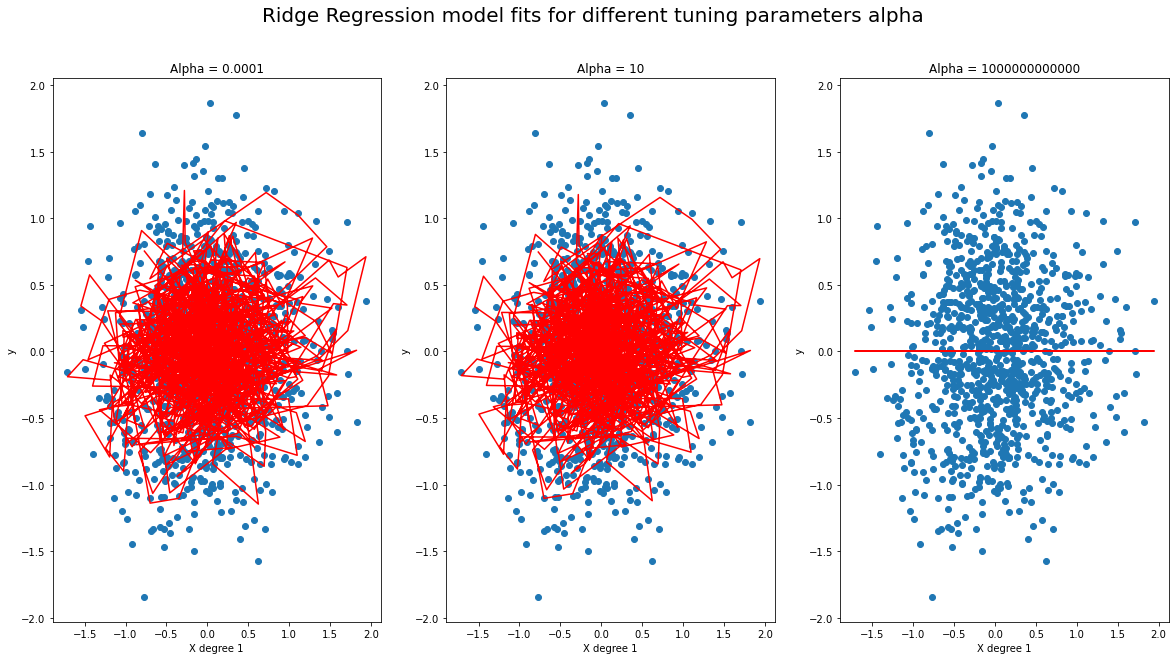
\includegraphics[width = 0.95\textwidth]{images/1.png}
    \caption{Ridge regression model fits for different tuning parameters $\lambda$}
    %\label{fig:mesh1}
\end{figure}

Then, we can move on the actual parameter and performance estimation  part via cross-validation technique. Cross-validation is a technique to evaluate predictive models by partitioning the original sample into a training set to train the model, and a test/val set to evaluate it.

\bigskip
In k-fold cross-validation, the original sample is randomly partitioned into k equal size subsamples. Of the k subsamples, a single subsample is retained as the validation data for testing the model, and the remaining k-1 subsamples are used as training data. The cross-validation process is then repeated k times (the folds), with each of the k subsamples used exactly once as the validation data. The k results from the folds can then be averaged (or otherwise combined) to produce a single estimation. The advantage of this method is that all observations are used for both training and validation, and each observation is used for validation exactly once. But note that in our case, we are asked to do a three-way split of the data, i.e.,  select a validation set of 100 contiguous samples, a testing set of 100 samples and a training set of length 800 samples.

\newpage
{\scshape EEE 482} \hfill {\scshape \large  Homework-\romannumeral3\relax} \hfill {\scshape Can Kocagil}
\smallskip
\hrule
\vspace{2mm}

To accomplish that, the following code snippted performs K-fold cross validation as a three-way split.
\begin{mintedbox}{python}
class K_fold(object):
    """
    Cross-validation, sometimes called rotation estimation or out-of-sample testing, is any of various similar model validation techniques for assessing how the results of a statistical analysis will generalize to an independent data set
    """
    def __init__(self,sample_size:int = y.shape[0], folds:int = 10):
        """
            Constructor method for initializing the sample size and the number of folds

                Arguments:
                    - sample_size (int) : How many samples are in the dataset
                    - folds (int) : the number of folds
        """
        
        self.sample_size = sample_size
        self.folds = folds
        self.fold_size = int(sample_size / folds)

    def split(self) -> tuple:
        """
            Generator function for splitting data as validation (10%), testing (10%) and training (80%) as K-fold cross validation based resampling
        """

        for idx in range(self.folds):
            _val_idx   = idx * self.fold_size
            _test_idx  = (idx + 1) * self.fold_size
            _train_idx = (idx + 2) * self.fold_size

            val_idx   = np.arange(_val_idx, _test_idx) % self.sample_size
            test_idx  = np.arange(_test_idx, _train_idx) % self.sample_size
            train_idx = np.arange(_train_idx, self.sample_size + _val_idx) % self.sample_size

            yield val_idx, test_idx, train_idx
\end{mintedbox}

Then, let's instantiate the K-fold class and perform 10-fold cross validation as follows.
\begin{mintedbox}{python}
dict_inference = {
    'test'  : dict(),
    'val'   : dict()
}


phases = [
    'train',
    'val',
    'test'
    
]

log_lambda_arr = np.logspace(
    start = 0,
    stop  = 12,
    num   = 500,
    base  = 10
)

cv = K_fold(folds = 10)

for val_idx, test_idx, train_idx in cv.split():

    X_list = [
        X[train_idx],
        X[val_idx],
        X[test_idx]
    ]

    y_list = [
        y[train_idx],
        y[val_idx],
        y[test_idx]
    ]


    for _lambda in log_lambda_arr:

        for phase, X_phase, y_phase in zip(phases, X_list, y_list):                               
            if phase == 'train':
                 model = RidgeRegression(_lambda)
                 model.fit(X_phase, y_phase) 

            else:                         
                preds = model.predict(X_phase)  
                r2_score = model.eval_r2(y_phase, preds)             
                dict_inference[phase].setdefault(
                    _lambda, list()).append(r2_score)               

inference_r2 = {
    phase : {      
        _lambda : np.mean(r2_score) for _lambda, r2_score in dict_inference[phase].items()  
    }                                                           
        for phase in ['val','test']     
}


\end{mintedbox}

\newpage
{\scshape EEE 482} \hfill {\scshape \large  Homework-\romannumeral3\relax} \hfill {\scshape Can Kocagil}
\smallskip
\hrule
\vspace{2mm}

At this point, I successfully estimate the $R^2$ on both validation and test. Additionally, I found the $\lambda_{opt}$ as follows.
\begin{mintedbox}{python}
best_r2 = 0
for _lambda, r_2 in inference_r2['val'].items():
    if r_2 > best_r2:
        best_r2 = r_2
        best_lambda = _lambda


print(f'Best lambda parameter that maximizes the R^2 is : {best_lambda}')
print('Best R^2 along the testing :', inference_r2['test'][best_lambda])
print('Best R^2 along the validation :', inference_r2['val'][best_lambda])
\end{mintedbox}

Best lambda parameter that maximizes the $R^2$ is : 395.5436244734702 \\
Best $R^2$ along the testing : 0.16042061044928463 \\ 
Best $R^2$ along the validation : 0.15259887784859996

\bigskip

Hence, we found $\lambda_{opt} = 395.543$. Let's visualize the inference progress through the cross-validation as a better intuition of how our ridge model estimate target variable w.r.t. varying parameter $\lambda$.

\begin{figure}[h]
    \centering
    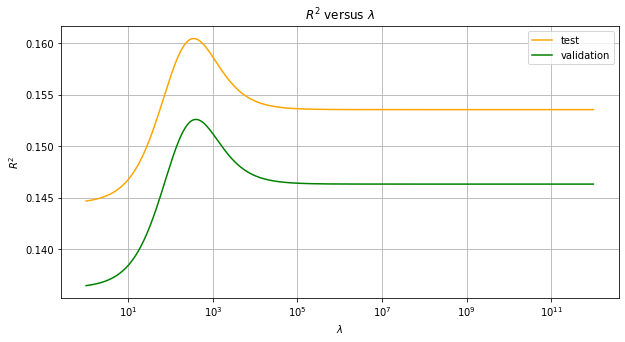
\includegraphics[width = 1\textwidth]{images/2.png}
    \caption{Ridge regression model fits for different tuning parameters $\lambda$ in the logarithmic sense}
    %\label{fig:mesh1}
\end{figure}

We can see from the figure that, there is a optimal $\lambda$, $\lambda_{opt}$ that maximizes the explained variance in the validation as well as testing phase. But, since validation data is used for estimating the model parameters, we choose the optimal parameter of the ridge model $\lambda_{opt}$ according to validation samples.

\newpage
{\scshape EEE 482} \hfill {\scshape \large  Homework-\romannumeral3\relax} \hfill {\scshape Can Kocagil}
\smallskip
\hrule
\vspace{2mm}

\subsection{Part B}

In this part of the question, we will determine confidence intervals for parameters of the OLS model from part a. OLS model corresponds to $\lambda = 0$ case in ridge regression so OLS model minimize the sum of squared error in the sense of statistical estimation. To do that, I generate bootstrap samples from the 1000 samples in the original data and perform 500 bootstrap iterations, and refit a separate model at each iteration. 

\bigskip

Bootstrapping is any test or metric that uses random sampling with replacement (e.g. mimicking the sampling process), and falls under the broader class of resampling methods \cite{enwiki:1014701581}. Bootstrapping assigns measures of accuracy (bias, variance, confidence intervals, prediction error, etc.) to sample estimates \cite{enwiki:1014701581}. This technique allows estimation of the sampling distribution of almost any statistic using random sampling methods \cite{enwiki:1014701581}

In our case, we generate bootstrap samples to estimate the $95\%$ confidence interval and to find statistically significant weights. So, let's see the Python code for bootstrapping. But before that, for reproducibility purposes, I create random seed operation as follows:

\begin{mintedbox}{python}
def random_seed(seed:int = 42) -> None :
    """ Random seeding for reproducibility 
    
            Arguments:
                - seed (int) : random state

            Returns:
                - None
    """
    np.random.seed(seed)
    random.seed(seed)
\end{mintedbox}

Then, here is code for bootstraping.
\begin{mintedbox}{python}
random_seed(10)

bootstrap_iters = range(500)
sample_idx = np.arange(X.shape[0])
parameters = list()

for idx in bootstrap_iters:

    bootstrap_idx = np.random.choice(sample_idx, size = 1000, replace = True)
    y_bootstrap = y[bootstrap_idx]
    X_bootstrap = X[bootstrap_idx]
    ridge = RidgeRegression(Lambda = 0)
    ridge.fit(X_bootstrap,y_bootstrap)
    parameters.append(ridge.parameters()) 
    
w_bootstrap = np.array(parameters)
w_mean = np.mean(w_bootstrap, axis=0)
w_std = np.std(w_bootstrap, axis=0)
\end{mintedbox}


So, what we done here is that we generate random indexes with replacement, then sample from our actual data, fit OLS model. After the completion of bootstrapping, we estimate model reliability by averaging the means of each bootstrap iteration. Then, we also calculate the standard deviation of sampling distribution of model parameter to compute test statistics in the following parts.

\newpage
{\scshape EEE 482} \hfill {\scshape \large  Homework-\romannumeral3\relax} \hfill {\scshape Can Kocagil}
\smallskip
\hrule
\vspace{2mm}

Then, let's move on the statistical test, confidence intervals and hypothesis testing part. Since, this assignment focused on the concept of  hypothesis testing, I will briefly describe the concept for future use and easy understanding by focusing on the concept not equations since every statistical test requires similar but different derivations to calculate confidence interval, etc.

\bigskip

A confidence interval is a range of values that is likely to contain an unknown population parameter. If you draw a random sample many times, a certain percentage of the confidence intervals will contain the population mean. This percentage is the confidence level. In our case, we will use confidence interval for OLS regression coefficients.


\bigskip
The relationship between p-values and confidence intervals can be interpreted as follows. In the context of hypothesis testing, one can use either p-values or confidence intervals to determine whether your results are statistically significant. If a hypothesis test produces both, these results will agree. As summary of relationship between p-value and confidence internal. We set type-I probability error term $\alpha$ and confidence level is equivalent to $1-\alpha$ level. Hence, if we predetermine significance level, for example 0.05, the corresponding confidence level yields $95\%$. Then, we can end up with
\smallskip

\begin{itemize}
    \item p-value $<$ $\alpha$ then the hypothesis test is statistically significant,
    \item If the confidence interval does not contain the null hypothesis value, the results are statistically significant
    \item  p-value $<$ $\alpha$ the confidence interval will not contain the null hypothesis value
\end{itemize}

\bigskip
Hence, we can interpret p-value as a significance level so that calculated value of a test statistic is borderline between rejection and acceptance region. Smaller p-values imply the rejection of null assumptions so they indicates research hypothesis is statistically significant. In other words, smaller p-values indicates strong evidence against the null hypothesis and also we can say that we get strong evidence for behoof of alternative hypothesis. Even the significance level changes study to study, researcher generally set 0.05 as the significance level so p-value $<$ 0.05 is small enough to say that alternative hypothesis is statistically significant.

\bigskip
Finally, we can move on our case. Then, here is code for plotting its mean and $95\%$ confidence interval in the sense of error plot.
\begin{mintedbox}{python}
plt.figure(figsize = (10,5))
plt.errorbar(np.arange(1, 101),
             w_mean,
             yerr= w_std,
             ecolor='red',
             elinewidth=1,
             capsize=1)
plt.title('Ridge Model OLS Weights')
plt.xlabel('i')
plt.ylabel('$W_i$')
plt.show()
\end{mintedbox}

\newpage
{\scshape EEE 482} \hfill {\scshape \large  Homework-\romannumeral3\relax} \hfill {\scshape Can Kocagil}
\smallskip
\hrule
\vspace{2mm}

\begin{figure}[h]
    \centering
    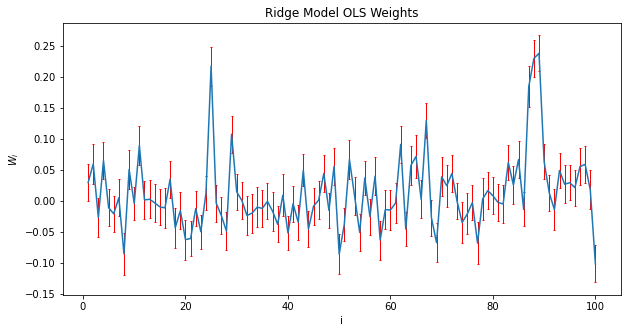
\includegraphics[width = 1\textwidth]{images/3.png}
    \caption{Ridge regression model weights for bootstrapped iterations and its $95\%$ confidence interval}
    %\label{fig:mesh1}
\end{figure}

Hence, to calculate p-value, we need to standardize our sampling distribution. So, here is the standardization and calculation of p-value with the indexes of statistically significant weights different than 0.

\begin{mintedbox}{python}
two_sided = 2
p_values = special.ndtr(- w_mean / w_std) * two_sided
alpha_level = 0.05
significants = np.argwhere(p_values < alpha_level).flatten()
print(f' Index of the parameters that are significantly different than 0: \n {significants}')
     
\end{mintedbox}

Index of the parameters that are significantly different than 0:  \\
 3 10 24 28 51 61 64 66 82 84 86 87 88 89 97


\subsection{Part C}
In this part of the question, we will determine confidence intervals for parameters of the regularized linear model from part a, i.e., the model obtained for $\lambda_{opt}$. To do that, as we done in the previous part, I generate bootstrap samples from the 1000 samples in the original data and perform 500 bootstrap iterations, and refit a separate model at each iteration using $\lambda_{opt}$. Then, I will plot the mean and 95\% confidence intervals of the parameters in the same graph with providing the model regressors which have weights that are significantly, different than 0.


\bigskip
Here is the Python code for generating bootstrapped samples.

\begin{mintedbox}{python}
random_seed(10)

bootstrap_iters = range(500)
sample_idx = np.arange(X.shape[0])
parameters = list()

for idx in bootstrap_iters:

    bootstrap_idx = np.random.choice(sample_idx, size = 1000, replace = True)
    y_bootstrap = y[bootstrap_idx]
    X_bootstrap = X[bootstrap_idx]
    ridge = RidgeRegression(Lambda = best_lambda)
    ridge.fit(X_bootstrap,y_bootstrap)
    parameters.append(ridge.parameters()) 
    
w_bootstrap = np.array(parameters)
w_mean = np.mean(w_bootstrap, axis=0)
w_std = np.std(w_bootstrap, axis=0)
\end{mintedbox}


Then, here is code for plotting its mean and $95\%$ confidence interval in the sense that error plot.
\begin{mintedbox}{python}
plt.figure(figsize = (10,5))
plt.errorbar(np.arange(1, 101),
             w_mean,
             yerr= w_std,
             ecolor='red',
             elinewidth=1,
             capsize=1)
plt.title('Ridge Model $\lambda_{optimal}$  Weights')
plt.xlabel('i')
plt.ylabel('$W_i$')
plt.show()
\end{mintedbox}

\begin{figure}[h]
    \centering
    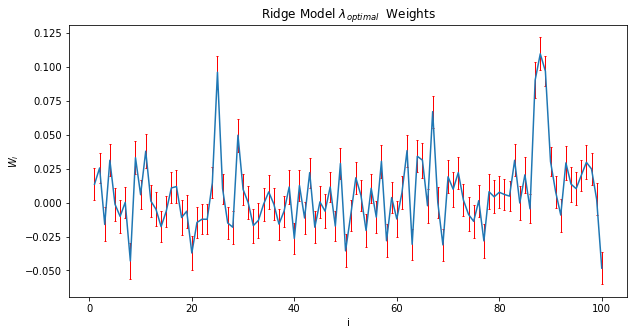
\includegraphics[width = 1\textwidth]{images/4.png}
    \caption{Ridge regression model weights for bootstrapped iterations and its $95\%$ confidence interval}
    %\label{fig:mesh1}
\end{figure}

\newpage
{\scshape EEE 482} \hfill {\scshape \large  Homework-\romannumeral3\relax} \hfill {\scshape Can Kocagil}
\smallskip
\hrule
\vspace{2mm}


Hence, to calculate p-value, we need to standardize our sampling distribution. So, here is the standardization and calculation of p-value with the indexes of statistically significant weights different than 0.

\begin{mintedbox}{python}
p_values = scipy.special.ndtr(- w_mean / w_std) * two_sided
significants = np.argwhere(p_values < alpha_level).flatten()
print(f' Index of the parameters that are significantly different than 0: \n {significants}')
      
\end{mintedbox}

Index of the parameters that are significantly different than 0: \\
 1  3  8 10 24 28 42 48 56 61 63 64 66 82 86 87 88 89 92 96 97

\bigskip

Hence, we can see that with the optimal Ridge model the number of indexes of the model regressors which have weights that are significantly different than 0 (at a significance level of p $<$ 0.05) is increased when compared to OLS. The reason behind this, we added penalty $L_{2-norm}$ term to the OLS estimator which stricts the parameters within smaller numbers w.r.t. OLS case with the increasing number of bootstraped samples. So, as we truly estimate the coefficient of the model, the number of parameters that are significantly different than 0 (with alpha level = 0.05) is increased.

\section{Question 2}
In this question, a series of neural response measurements are provided in the file hw3\_data3.mat.

\subsection{Part A}
In this part, responses from two separate populations of neurons are stored in the variables pop1 and pop2. We would like to examine whether the mean responses of the two populations are significantly different. In other words, we examine if they are drawn from the same distribution or not with alpha level = 0.05. As a prior information to the researcher, the first population contains 7 neurons, whereas the second population contains 5 neurons. 

\bigskip

To test our null hypothesis that states that two datasets follow the same distribution versus the alternative that indicates the just the opposite of null hypothesis (two-tailed) with alpha level = 0.05. Let's construct the hypothesis testing formulation as follows. Let $\mu_1$ and $\mu_2$ represents the means of pop1 and pop2 respectively such that

\begin{align*}
    \textit{Null hypothesis } H_o : \mu_1 - \mu_2 = 0 
    \textit{ and researcher hypothesis } H_a : \mu_1 - \mu_2 \	\neq 0
\end{align*}

So, we priory believe that our responses are coming from the same distribution so that there is no such underlying mean difference in the sense of statistical estimation. Now, we will test our hypothesis versus alternative one as follows.

\bigskip
In the question, there is a hint that says if the two datasets come from a common distribution, is there any need to separate
them. So, we priory assume that there is no separation between the the pop1 and pop2 so we can combine in a single population as first step of hypothesis testing. Then, we need to bootstrap the data with 10 000 iteration to estimate its sampling distribution and characterization of its test-statistics. Here is the Python code for bootstrapping.


\newpage
{\scshape EEE 482} \hfill {\scshape \large  Homework-\romannumeral3\relax} \hfill {\scshape Can Kocagil}
\smallskip
\hrule
\vspace{2mm}


\begin{mintedbox}{python}
def bootstrap(sample:np.ndarray, bootstrap_iters:iter = range(10000), random_state:int = 11) -> np.ndarray:
    """
    
        Generate bootstrap samples using random sampling with replacement.
        
            Arguments:
                - sample (np.ndarray) : Sample to be bootstraped
                - bootstrap_iters (iterator object) : Specification of bootstrap iterations
                - random_state (int) : Random seed for reproducibility

            Returns:
                - bootstrap_samples (np.ndarray) : Bootstrapped array

    """
    random_seed(random_state)
    size = sample.shape[0]
    bootstrap_samples = list()

    for idx in bootstrap_iters:        
        bootstrap_idx = np.random.choice(np.arange(sample.shape[0]), size = size, replace = True)
        bootstrap_samples.append(sample[bootstrap_idx])
    
    return np.array(bootstrap_sample
\end{mintedbox}

Then, I as mentioned, I aggregated the pop1 and pop2 in column wise. Then, I bootstrapped from that aggregated samples. Next step is select 7 values from  sample and represent the values as first populations responses. In the same manner, we interpret the remaining 5 values of each sample as second populations responses. Since, as a priory, we believe that they come from the same underlying distribution so there is no discrepancy to claim in this manner. Hence, we compute difference of means by subtracting the representation of first population with bootstrapped samples from second one. Then, here is the code for computation of difference of means and its visualization.

\begin{mintedbox}{python}
pop = np.vstack([pop1,pop2])
pop_bootstrap = bootstrap(pop)
sample_1 = pop_bootstrap[:,:len(pop1)].squeeze(2)
sample_2 = pop_bootstrap[:,len(pop1):].squeeze(2)
sample_1_bootstrap_mean = sample_1.mean(axis = 1)
sample_2_bootstrap_mean = sample_2.mean(axis = 1)
sample_diff_means = sample_1_bootstrap_mean - sample_2_bootstrap_mean
sample_mean_dist = pd.DataFrame()
sample_mean_dist['Mean Difference'] = sample_diff_means.flatten()
fig, ax = plt.subplots(figsize = (10,5))
sample_mean_dist.plot.kde(ax=ax, title='Difference of Means of Bootstrapped Populations 1 and 2')
sample_mean_dist.plot.hist(density=True, ax = ax, bins = 15)
ax.set_ylabel('Probability $P_X(x)$')
ax.set_xlabel('Difference in means (x)')
ax.grid(axis='y')
ax.set_yticks([])
\end{mintedbox}

\newpage
{\scshape EEE 482} \hfill {\scshape \large  Homework-\romannumeral3\relax} \hfill {\scshape Can Kocagil}
\smallskip
\hrule
\vspace{2mm}

\begin{figure}[h]
    \centering
    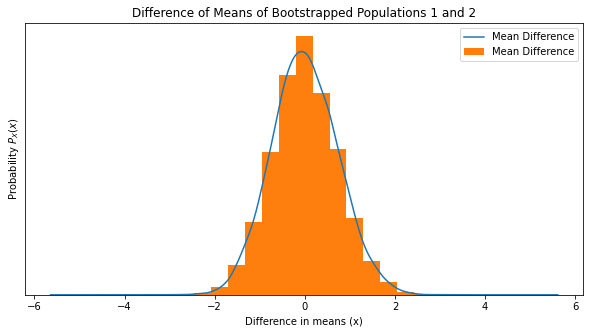
\includegraphics[width = 1\textwidth]{images/5.png}
    \caption{Difference of Means of Bootstrapped Populations 1 and 2}
    %\label{fig:mesh1}
\end{figure}

Here, the figure represents our sampling distribution of difference of means. As we can see, it is almost zero centered Gaussian. Let's analyze the sampling distribution of the pop1 and pop2 separately to compare above figure as it is very intuitive way of understanding of the problem. Let's see the corresponding code and the figures.


\begin{mintedbox}{python}
pop1_bootstrap = bootstrap(pop1)
pop2_bootstrap = bootstrap(pop2)
pop1_bootstrap_mean = np.mean(pop1_bootstrap, axis = 1)
pop2_bootstrap_mean = np.mean(pop2_bootstrap, axis = 1)

mean_dist = pd.DataFrame()
mean_dist['pop1 Mean'] = pop1_bootstrap_mean.flatten()
mean_dist['pop2 Mean'] = pop2_bootstrap_mean.flatten()
mean_dist['Mean Difference'] = pop1_bootstrap_mean - pop2_bootstrap_mean

fig, ax = plt.subplots(figsize = (10,5))
mean_dist.plot.kde(ax=ax, title='Difference of Means of Bootstrapped Populations 1 and 2')
mean_dist.plot.hist(density=True, ax = ax, bins = 15)
ax.set_ylabel('Probability $P_X(x)$')
ax.set_xlabel('Difference in means (x)')
ax.grid(axis='y')
ax.set_yticks([])
\end{mintedbox}

\newpage
{\scshape EEE 482} \hfill {\scshape \large  Homework-\romannumeral3\relax} \hfill {\scshape Can Kocagil}
\smallskip
\hrule
\vspace{2mm}

\begin{figure}[h]
    \centering
    
\includegraphics[width = 1\textwidth]{images/6.png}
    \caption{Difference of Means of Bootstrapped Populations 1 and 2}
    %\label{fig:mesh1}
\end{figure}

Hence, before the calculation of the p-value and test statistic, we get the intuition that the actual bootstrapped difference of means centered around 2 whereas the null hypothesis statements centered around 0. 

Then, let's calculate test statistic and p-value to test our hypothesis as follows.
\begin{mintedbox}{python}
actual_diff_means = pop1.mean() - pop2.mean()
std_test = sample_mean_dist['Mean Difference'].std()
mean_test = sample_mean_dist['Mean Difference'].mean()

z_cal = (mean_test - actual_diff_means) / std_test
p_values = scipy.special.ndtr(z_cal) * two_sided

print('The two sided p-value is:', p_values)
\end{mintedbox}

The two sided p-value is: 0.01003287406404004

\bigskip

As we can see, p-value $<$ alpha level that indicates the rejection of our prior believes about the population, i.e., null hypothesis. Hence, researcher find a strong evidence to indicate the rejection of prior believe that pop1 and pop2 are drawn from the same distribution. Hence, researcher hypothesis is statistically significant.

\subsection{Part B}
In this part, BOLD responses recorded in two voxels in the human brain are stored in the variables vox1 and vox2 and we would like to examine whether the voxel responses are similar to each other, by calculating their correlation. As done in the previous parts, I will find the mean and $95\%$ confidence interval by bootstrapping 10 000 iterations. Then, I will find the percentile of the bootstrap distribution, corresponding to a correlation value of 0.

\bigskip

Here, we bootstrapped the vox1 and vox2 separately as our prior believe they are not correlated in the sense of Pearson. Hence, our null hypothesis implies that the distributions vox1 and vox2 are not correlated.

\newpage
{\scshape EEE 482} \hfill {\scshape \large  Homework-\romannumeral3\relax} \hfill {\scshape Can Kocagil}
\smallskip
\hrule
\vspace{2mm}

In the context of hypothesis testing, researcher hypothesis implies the correlation between vox1 and vox2. Let's look at the sampling distribution of the correlation between vox1 and vox2, then calculate test statistic to test our prior believe under the null assumption as follows. Note that since the null hypothesis is not given directly, either ways of computing the end result should agree. 

\begin{mintedbox}{python}
def corr(X:np.ndarray,Y:np.ndarray) -> list:
    """
        Given the X,Y distributions, computes the correlation element wise.
    
            Arguments:
                - X (list or np.ndarray) : First distribution
                - Y (list or np.ndarray) : Second distribution

            Returns:
                - pearson_corrs (list[float]) : Correlations element wise
    """
    return [scipy.stats.pearsonr(X[i], Y[i])[0] for i in range(X.shape[0])]
    
vox1_bootstrap = bootstrap(vox1)
vox2_bootstrap = bootstrap(vox2)
corr_bootstrap = corr(vox1_bootstrap,vox2_bootstrap)
fig, ax = plt.subplots(figsize = (10,5))
pd.Series(corr_bootstrap).plot.kde(ax=ax, legend = False, title='Sampling Distribution of Correlation between vox1 and vox2')
pd.Series(corr_bootstrap).plot.hist(density=True, ax = ax, bins = 20, alpha = 0.8,color = 'red')
ax.set_ylabel('Probability $P_Y(y)$')
ax.set_xlabel('Pearson Correlation y')
ax.grid(axis='y')
ax.set_yticks([])
\end{mintedbox}

\begin{figure}[h]
    \centering
    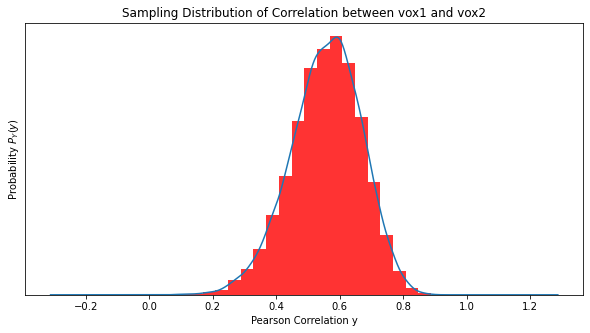
\includegraphics[width = 0.9\textwidth]{images/8.png}
    \caption{Sampling distribution of correlation between vox1 and vox2}
    %\label{fig:mesh1}
\end{figure}



\newpage
{\scshape EEE 482} \hfill {\scshape \large  Homework-\romannumeral3\relax} \hfill {\scshape Can Kocagil}
\smallskip
\hrule
\vspace{2mm}

As we can see from the figure, sampling distribution of correlation between vox1 and vox2 have correlation centered around 0.55 as a first intuition of our test progress. It seems we will find enough evidence against our null assumptions such that rejection of null hypothesis is likely. Then, let's calculate mean and $95\%$ confidence interval as follows.


\begin{mintedbox}{python}
# Thanks to 
# https://stackoverflow.com/questions/15033511/
# compute-a-confidence-interval-from-sample-data
def confidence_interval(data:np.ndarray, confidence:float=0.95) -> tuple:
    """
        Given the distribution and confidence level, computes the confidence interval.
            
            Arguments:
                - data (list or np.ndarray) : Input distribution
                - confidence (float) : confidence level in the range [0,1]
            
            Returns:
                - confidence_level (tuple[np.ndarray]) : lower, upper limits respectively
    """
    a = 1.0 * np.array(data)
    n = len(a)
    m, se = np.mean(a), scipy.stats.sem(a)
    h = se * scipy.stats.t.ppf((1 + confidence) / 2., n-1)
    return m-h, m+h
    
corr_mean = np.mean(corr_bootstrap)
lower, upper = confidence_interval(corr_bootstrap,confidence=0.95)
print('Mean correlation value:', corr_mean)
print(f'95% confidence interval of the correlation values: {lower, upper}')
\end{mintedbox}

Mean correlation value: 0.5571443738567518 \\
95\% confidence interval of the correlation values: (0.5549693272197517, 0.5593194204937518)

\bigskip

As we previously analyze the distribution of sampling correlation and conclude that expected correlation is around 0.55 and our actual mean correlation of sampling distribution value is found as 0.557. 

\bigskip
After that, we are asked to find the percentile of the bootstrap distribution, corresponding to a correlation value of 0. But, since we already got enough evidence against our null assumptions and analyzed the bootstrapped and mean correlation and conclude that vox1 and vox2 is correlated and this correlation is centered around 0.55, we expect little or no percentile of the bootstrap distribution, corresponding to a correlation value of 0. Let's find direct percentage through the Python as follows.

\begin{mintedbox}{python}
is_corr_zero = np.argwhere(corr_bootstrap == 0)
corr_zero_percentage = 100 * is_corr_zero.shape[0] / 10000
print('Percentage of zero correlation values:', corr_zero_percentage)
\end{mintedbox}

Percentage of zero correlation values: 0.0

\bigskip

As our intuition, and direct calculation of the percentile of the bootstrap distribution, corresponding to a correlation value of 0 indicates that its value is zero.


\newpage
{\scshape EEE 482} \hfill {\scshape \large  Homework-\romannumeral3\relax} \hfill {\scshape Can Kocagil}
\smallskip
\hrule
\vspace{2mm}

\subsection{Part C}
As the question implies estimation of confidence intervals and hypothesis testing are dual problems, we already have good enough intuition about this question and the evidence against the null hypothesis. But, for the sake of the question indicates the computation of break apart correlation of bootstrapped samples, let's visualize the sampling distribution and compute p-value for two voxels having zero or negative correlation. Let's see the code and visualization for part C in one shot.


\begin{mintedbox}{python}
vox1_ind = bootstrap(vox1, range(10000), random_state=42)
vox2_ind = bootstrap(vox2, range(10000), random_state=21)

_corr_ind = corr(vox1_ind,vox2_ind)
corr_ind = pd.Series(_corr_ind)

fig, ax = plt.subplots(figsize = (10,5))
corr_ind.plot.kde(ax=ax, legend = False, title='Sampling Distribution of Correlation between vox1 and vox2')
corr_ind.plot.hist(density=True, ax = ax, bins = 20, alpha = 0.8,color = 'red')
ax.set_ylabel('Probability $P_Y(y)$')
ax.set_xlabel('Pearson Correlation y')
ax.grid(axis='y')
ax.set_yticks([])

actual_corr, _ = scipy.stats.pearsonr(vox1,vox2)
mean_corr = corr_ind.mean()
std_corr = corr_ind.std()
z_score = mean_corr - actual_corr
z_score /= std_corr
p_value = scipy.special.ndtr(z_score)
print('The one sided p-value is:', p_value)
\end{mintedbox}



\begin{figure}[h]
    \centering
    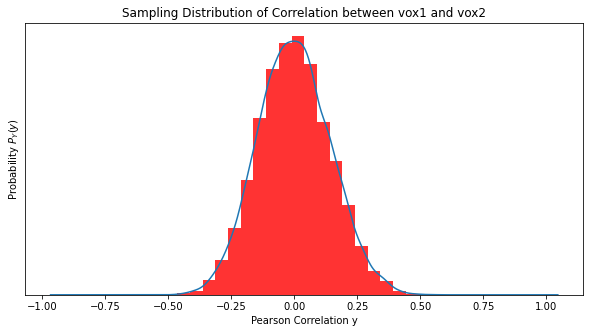
\includegraphics[width = 1\textwidth]{images/9.png}
    \caption{Sampling distribution of correlation between vox1 and vox2}
    %\label{fig:mesh1}
\end{figure}


\newpage
{\scshape EEE 482} \hfill {\scshape \large  Homework-\romannumeral3\relax} \hfill {\scshape Can Kocagil}
\smallskip
\hrule
\vspace{2mm}

The one sided p-value is: 3.812065700707869e-05

\bigskip

As our intuition and calculated p-value indicates that (p-value $<$ alpha level) we have a strong evidence against the null assumption that states that  two voxel responses have zero or negative correlation so that we reject our null hypothesis.

\subsection{Part D}
In this part of the question, the average BOLD responses in a face-selective region of the human brain have been
recorded in two separate experiments. The responses of this region to building images ($1^{st}$ experiment) and face images ($2^{nd}$ experiment) are stored in the variables building and face for 20 subjects. Additionally, there is prior assumption that the same subject population was recruited in both experiments. We need to use bootstrapping (10000 iterations) to calculate the two-tailed p-value for the null hypothesis that there is no difference between the building and face responses.

\bigskip
In the underlying conditions, our prior believe is that there is no difference between the building and face as it is our null hypothesis. Also, researcher/alternative hypothesis is just the opposite so that our hypothesis procedure requires two-tailed p-value calculation. However, in these case, the situation is bit different than the previous ones as we have have an assumption that the subjects are the same for both experiments. We need to generate single difference of means. Our subject can be faced with $2^2 = 4$ cases which are
\smallskip

\begin{itemize}
    \item Face, Face
    \item Face, Building
    \item Building, Face
    \item Building, Building
\end{itemize}

Hence, to generate unbiased experiment in statistical sense we need to generate samples by choosing 4 cases with the number of bootstrap iteration. Things will be more clear with the code part as it is placed below.

\begin{mintedbox}{python}
random_seed(31)

assert building.shape[0] == face.shape[0],'Dimensionality Mismatch!'

sample_size = np.arange(building.shape[0])

_mean_diff = list()
bootstrap_iters  = np.arange(10000)

for ii in bootstrap_iters:
    
    resample = []
    
    for jj in sample_size:
        
        bootstrap_idx = np.random.choice(np.arange(building.shape[0]), replace = True)
        options = [0] * 2
        _option = building[jj] - face[jj]
        options.append(_option)
        _option = face[jj] - building[jj]
        options.append(_option)
        resample.append(np.random.choice(options))
        
    _mean_diff.append(np.mean(resample))

\end{mintedbox}

\newpage
{\scshape EEE 482} \hfill {\scshape \large  Homework-\romannumeral3\relax} \hfill {\scshape Can Kocagil}
\smallskip
\hrule
\vspace{2mm}

Here, I bootstrapped samples according to our underlying situation and calculate the difference of means in. Let's look at the distribution of difference of means of follows.

\begin{mintedbox}{python}
mean_diff = pd.Series(_mean_diff)
fig, ax = plt.subplots(figsize = (10,5))
mean_diff.plot.kde(ax=ax, legend = False, title='Difference in means of building and face')
mean_diff.plot.hist(density=True, ax = ax, bins = 40, alpha = 0.8, color = 'red')
ax.set_ylabel('Probability $P_X(x)$')
ax.set_xlabel('Difference in means (x)')
ax.grid(axis='y')
ax.set_yticks([])

\end{mintedbox}

\begin{figure}[h]
    \centering
    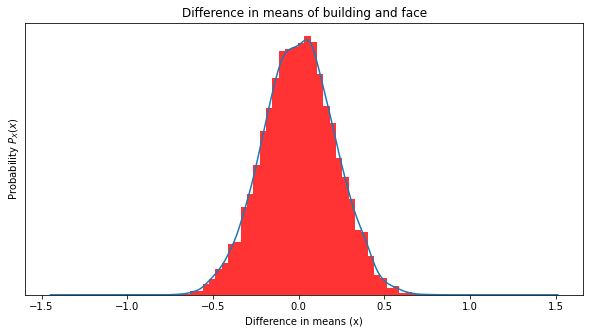
\includegraphics[width = 1\textwidth]{images/10.png}
    \caption{Sampling distribution of difference of means of building and face}
    %\label{fig:mesh1}
\end{figure}

The shape of the distribution implies zero centered Gaussian. Let's test our hypothesis by calculating test statistic and p-value as follows.

\begin{mintedbox}{python}
x_actual = np.mean(building) - np.mean(face)
mean = mean_diff.mean()
std = mean_diff.std()
z_score = mean - x_actual
z_score /= std
p_value = scipy.special.ndtr(- z_score) * two_sided
print('The two sided p-value is:', p_value)
\end{mintedbox}

The two sided p-value is: 0.000356527118064005
\bigskip

As p-value indicates rejection of our prior believe that there is no difference between the building and face since it is much smaller than our alpha level (0.05). Hence, we kindly reject our null hypothesis as we found strong evidence against it and conclude that the hypothesis that states there is difference between the building and face responses are statistically significant. 

\newpage
{\scshape EEE 482} \hfill {\scshape \large  Homework-\romannumeral3\relax} \hfill {\scshape Can Kocagil}
\smallskip
\hrule
\vspace{2mm}


\subsection{Part E}
In this part, we are asked to repeat the exercise in part d, but this time assuming that the subject populations
recruited for the two experiments are distinct. To do that, we will bootstrap (10000 iterations) to calculate the two-tailed p-value for the null hypothesis that there is no difference between the building and face responses. 

\bigskip
Here is Python code for computation of it sampling distribution, visualization of its discretized density and p-value.

\begin{mintedbox}{python}
arr_stack = np.hstack((building, face))
arr_bootstrap = bootstrap(arr_stack)
samples1 = arr_bootstrap[:, :len(building)]
samples2 = arr_bootstrap[:, len(building):]
means1 = np.mean(samples1, axis=1)
means2 = np.mean(samples2, axis=1)
sample_diff_means = means1 - means2
\end{mintedbox}

At this point, difference of means are calculated, let's visualize the distribution as follows.

\begin{mintedbox}{python}
sample_mean_dist = pd.DataFrame()
sample_mean_dist['Mean Difference'] = sample_diff_means.flatten()
fig, ax = plt.subplots(figsize = (10,5))
sample_mean_dist.plot.kde(ax=ax, title='Difference of Means of Bootstrapped Populations building and face')
sample_mean_dist.plot.hist(density=True, ax = ax, bins = 50)
ax.set_ylabel('Probability $P_X(x)$')
ax.set_xlabel('Difference in means (x)')
ax.grid(axis='y')
ax.set_yticks([])
\end{mintedbox}


\begin{figure}[h]
    \centering
    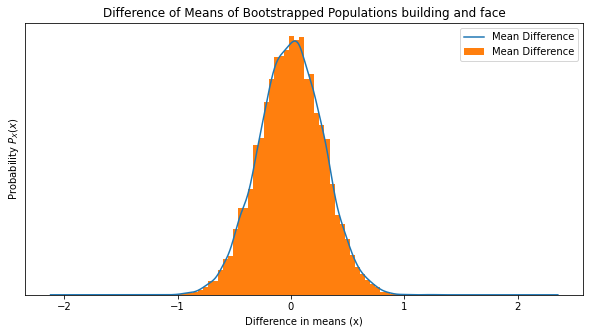
\includegraphics[width = 1\textwidth]{images/11.png}
    \caption{Sampling distribution of difference of means of building and face}
    %\label{fig:mesh1}
\end{figure}

\newpage
{\scshape EEE 482} \hfill {\scshape \large  Homework-\romannumeral3\relax} \hfill {\scshape Can Kocagil}
\smallskip
\hrule
\vspace{2mm}

\begin{mintedbox}{python}
x_actual = np.mean(building) - np.mean(face)
mean = sample_mean_dist.mean()
std = sample_mean_dist.std()
z_score = mean - x_actual
z_score /= std
p_value = scipy.special.ndtr(- z_score) * two_sided
print('The two sided p-value is:', p_value)
\end{mintedbox}

The one sided p-value is: Mean Difference    0.00844

\bigskip

Hence, corresponding p-value is calculated as 0.00844 that implies strong evidence agains to null hypothesis since it smaller than alpha level so that we reject our prior believe that that there is no difference between the building and face responses.

\newpage
{\scshape EEE 482} \hfill {\scshape \large  Homework-\romannumeral3\relax} \hfill {\scshape Can Kocagil}
\smallskip
\hrule
\vspace{2mm}

\section{Source Code}

\begin{mintedbox}{python}
#!/usr/bin/env python
# coding: utf-8

# In[19]:


import numpy as np
import matplotlib.pyplot as plt
import h5py
import scipy
import pandas as pd
import scipy.special as special
import random


# In[20]:


#cd D:\ThisSemester\CompNeuro\Homeworks\Hw3\HW3_Can_Kocagil\Assignment


# ### Question 1

# In[21]:


f = h5py.File('hw3_data2.mat','r')

X = np.array(f.get('Xn')).T

y = np.array(f.get('Yn')).flatten()
    
print(X.shape,y.shape)


# In[22]:


def random_seed(seed:int = 42) -> None :
    """ Random seeding for reproducebility 
    
            Arguments:
                - seed (int) : random state

            Returns:
                - None
    
    """
    np.random.seed(seed)
    random.seed(seed)


# In[23]:


class RidgeRegression(object):
    
    """
        Ridge regression is a method of estimating the coefficients of multiple-regression models in
        scenarios where independent variables are highly correlated. 

    """
    def __init__(self,Lambda:float=1):
        """
            Constructer method for initilization of ridge regression model.
            
            
                Arguments:
                    - Lambda (float): is the parameter which balances the amount 
                     of emphasis given to minimizing RSS vs minimizing sum of square of coefficients

        
        """

        self.Lambda = Lambda      
     
    def fit(self, X:np.ndarray, y:np.ndarray) -> None:
        """
            
            Given the pair of X,y, fit the data, i.e., find parameter W such that sum of square error
            is minimized. 
            

                Arguments:
                    - X (np.ndarray) : Regressor data 
                    - X (np.ndarray) : Ground truths for regressors

                Returns:
                    - None
        
        """
               
        I = np.eye(X.shape[1])
        
        self.W = np.linalg.inv(
            X.T.dot(X) + self.Lambda * I
            ).dot(X.T).dot(y)

        return self

    def predict(self,X:np.ndarray) -> np.ndarray :
        """
            Given the test data X, we predict the target variable.
            
                Arguments:
                    - X (np.ndarray) : The independant variable (regressor)

                Returns:
                    - Y_hat (np.ndarray) : Estimated value of y

        """
              
        return X.dot(self.W)
    
  
    def parameters(self) -> None:
        """
            Returns the estimated parameter W of the Ridge Regression
        
        """
        return self.W

    def eval_r2(self,y_true:np.ndarray, y_pred:np.ndarray) -> np.float:
        """
            Given the true dependant variable and estimated variable, computes proportion of
            explained variance R^2 by square the Pearson correlation between true dependant
            variable and estimated variabl
            
                Arguments:
                    - y_true (np.ndarray) : true dependant variable
                    - y_pred (np.ndarray) : estimated variable
                    
                Returns:
                    - r_squared (np.float) : Proportion of explained variance
        
        """

        _pearson = np.corrcoef(y_true,y_pred)
        pearson = _pearson[1][0]
        r_squared = np.square(pearson)
        return r_squared

    @staticmethod
    def R2(y_true:np.ndarray,y_pred:np.ndarray) -> np.float:
        r_squared = (1 - (sum((y_true - (y_pred))**2) / ((len(y_true) - 1) * np.var(y_true.T, ddof=1)))) * 100
        return r_squared


    def __str__(self):
        model = RidgeRegression().__class__.__name__
        model += f" with parameter \n"
        model += f"{self.Lambda}"
        return model


    def __repr__(self):
        model = RidgeRegression().__class__.__name__
        model += f" with parameter \n"
        model += f"{self.Lambda}"
        return model


# In[24]:


class K_fold(object):
    """
    Cross-validation, sometimes called rotation estimation or out-of-sample testing,
    is any of various similar model validation techniques for assessing how the results
    of a statistical analysis will generalize to an independent data set
    
    
    """
    def __init__(self,sample_size:int = y.shape[0], folds:int = 10):
        """
            Constructor method for initializing the sample size and the number of folds

                Arguments:
                    - sample_size (int) : How many samples are in the dataset
                    - folds (int) : the number of folds

        """
        
        self.sample_size = sample_size
        self.folds = folds
        self.fold_size = int(sample_size / folds)

    def split(self):
        """
            
            Generator function for splitting data as validation (10%), testing (10%) and
            training (80%) as K-fold cross validation based resampling
     
        """

        for idx in range(self.folds):
            _val_idx   = idx * self.fold_size
            _test_idx  = (idx + 1) * self.fold_size
            _train_idx = (idx + 2) * self.fold_size

            val_idx   = np.arange(_val_idx, _test_idx) % self.sample_size
            test_idx  = np.arange(_test_idx, _train_idx) % self.sample_size
            train_idx = np.arange(_train_idx, self.sample_size + _val_idx) % self.sample_size

            yield val_idx, test_idx, train_idx


# In[26]:


dict_inference = {
    'test'  : dict(),
    'val'   : dict()
}


phases = [
    'train',
    'val',
    'test'
    
]

log_lambda_arr = np.logspace(
    start = 0,
    stop  = 12,
    num   = 500,
    base  = 10
)

cv = K_fold(folds = 10)

for val_idx, test_idx, train_idx in cv.split():

    X_list = [
        X[train_idx],
        X[val_idx],
        X[test_idx]
    ]

    y_list = [
        y[train_idx],
        y[val_idx],
        y[test_idx]
    ]


    for _lambda in log_lambda_arr:

        for phase, X_phase, y_phase in zip(phases, X_list, y_list):                               
            if phase == 'train':
                 model = RidgeRegression(_lambda)
                 model.fit(X_phase, y_phase) 

            else:                         
                preds = model.predict(X_phase)  
                r2_score = model.eval_r2(y_phase, preds)             
                dict_inference[phase].setdefault(
                    _lambda, list()).append(r2_score)               

inference_r2 = {
    phase : {      
        _lambda : np.mean(r2_score) for _lambda, r2_score in dict_inference[phase].items()  
    }                                                           
        for phase in ['val','test']     
}


# In[27]:


best_r2 = 0
for _lambda, r_2 in inference_r2['val'].items():
    if r_2 > best_r2:
        best_r2 = r_2
        best_lambda = _lambda


print(f'Best lambda parameter that maximizes the R^2 is : {best_lambda}')
print('Best R^2 along the testing :', inference_r2['test'][best_lambda])
print('Best R^2 along the validation :', inference_r2['val'][best_lambda])


# In[28]:


lists1 = sorted(inference_r2['val'].items()) 
x1, y1 = zip(*lists1) 
lists2 = sorted(inference_r2['test'].items()) 
x2, y2 = zip(*lists2) 
plt.figure(figsize = (10,5))
plt.plot(x2, y2, color='orange')
plt.plot(x1, y1, color='g')
plt.legend(['test', 'validation'])
plt.ylabel('$R^2$')
plt.xlabel('$\lambda$')
plt.title('$R^2$ versus $\lambda$')
plt.xscale('log')
plt.grid()
plt.show()


# In[29]:


random_seed(10)

bootstrap_iters = range(500)
sample_idx = np.arange(X.shape[0])
parameters = list()

for idx in bootstrap_iters:

    bootstrap_idx = np.random.choice(sample_idx, size = 1000, replace = True)
    y_bootstrap = y[bootstrap_idx]
    X_bootstrap = X[bootstrap_idx]
    ridge = RidgeRegression(Lambda = 0)
    ridge.fit(X_bootstrap,y_bootstrap)
    parameters.append(ridge.parameters()) 
    
w_bootstrap = np.array(parameters)
w_mean = np.mean(w_bootstrap, axis=0)
w_std = np.std(w_bootstrap, axis=0)


# In[30]:


plt.figure(figsize = (10,5))
plt.errorbar(np.arange(1, 101),
             w_mean,
             yerr= w_std,
             ecolor='red',
             elinewidth=1,
             capsize=1)
plt.title('Ridge Model OLS Weights')
plt.xlabel('i')
plt.ylabel('$W_i$')
plt.show()


# In[31]:


two_sided = 2
p_values = special.ndtr(- w_mean / w_std) * two_sided
alpha_level = 0.05
significants = np.argwhere(p_values < alpha_level).flatten()
print(f' Index of the parameters that are significantly different than 0: \n {significants}')
     


# In[32]:


random_seed(10)

bootstrap_iters = range(500)
sample_idx = np.arange(X.shape[0])
parameters = list()

for idx in bootstrap_iters:

    bootstrap_idx = np.random.choice(sample_idx, size = 1000, replace = True)
    y_bootstrap = y[bootstrap_idx]
    X_bootstrap = X[bootstrap_idx]
    ridge = RidgeRegression(Lambda = best_lambda)
    ridge.fit(X_bootstrap,y_bootstrap)
    parameters.append(ridge.parameters()) 
    
w_bootstrap = np.array(parameters)
w_mean = np.mean(w_bootstrap, axis=0)
w_std = np.std(w_bootstrap, axis=0)


# In[33]:


plt.figure(figsize = (10,5))
plt.errorbar(np.arange(1, 101),
             w_mean,
             yerr= w_std,
             ecolor='red',
             elinewidth=1,
             capsize=1)
plt.title('Ridge Model $\lambda_{optimal}$  Weights')
plt.xlabel('i')
plt.ylabel('$W_i$')
plt.show()


# In[34]:


p_values = scipy.special.ndtr(- w_mean / w_std) * two_sided
significants = np.argwhere(p_values < alpha_level).flatten()
print(f' Index of the parameters that are significantly different than 0: \n {significants}')
     


# ### Question 2

# ## Part A

# In[44]:


f = h5py.File('hw3_data3.mat','r')
  
pop1 = np.array(
    f.get('pop1')
    )

pop2 = np.array(
    f.get('pop2')
    )


# In[45]:


def bootstrap(sample:np.ndarray, bootstrap_iters:iter = range(10000), random_state:int = 11) -> np.ndarray:
    """
    
        Generate bootstrap samples using random sampling with replacement.
        
            Arguments:
                - sample (np.ndarray) : Sample to be bootstraped
                - bootstrap_iters (iterator object) : Specification of bootstrap iterations
                - random_state (int) : Random seed for reproducibility

            Returns:
                - bootstrap_samples (np.ndarray) : Bootstrapped array

    """
    random_seed(random_state)
    size = sample.shape[0]
    bootstrap_samples = list()

    for idx in bootstrap_iters:        
        bootstrap_idx = np.random.choice(np.arange(sample.shape[0]), size = size, replace = True)
        bootstrap_samples.append(sample[bootstrap_idx])
    
    return np.array(bootstrap_samples)


# In[46]:


pop = np.vstack([pop1,pop2])
pop_bootstrap = bootstrap(pop)
sample_1 = pop_bootstrap[:,:len(pop1)].squeeze(2)
sample_2 = pop_bootstrap[:,len(pop1):].squeeze(2)
sample_1_bootstrap_mean = sample_1.mean(axis = 1)
sample_2_bootstrap_mean = sample_2.mean(axis = 1)
sample_diff_means = sample_1_bootstrap_mean - sample_2_bootstrap_mean
sample_mean_dist = pd.DataFrame()
sample_mean_dist['Mean Difference'] = sample_diff_means.flatten()
fig, ax = plt.subplots(figsize = (10,5))
sample_mean_dist.plot.kde(ax=ax, title='Difference of Means of Bootstrapped Populations 1 and 2')
sample_mean_dist.plot.hist(density=True, ax = ax, bins = 15)
ax.set_ylabel('Probability $P_X(x)$')
ax.set_xlabel('Difference in means (x)')
ax.grid(axis='y')
ax.set_yticks([])


# In[47]:


pop1_bootstrap = bootstrap(pop1)
pop2_bootstrap = bootstrap(pop2)
pop1_bootstrap_mean = np.mean(pop1_bootstrap, axis = 1)
pop2_bootstrap_mean = np.mean(pop2_bootstrap, axis = 1)

mean_dist = pd.DataFrame()
mean_dist['pop1 Mean'] = pop1_bootstrap_mean.flatten()
mean_dist['pop2 Mean'] = pop2_bootstrap_mean.flatten()
mean_dist['Mean Difference'] = pop1_bootstrap_mean - pop2_bootstrap_mean

fig, ax = plt.subplots(figsize = (10,5))
mean_dist.plot.kde(ax=ax, title='Difference of Means of Bootstrapped Populations 1 and 2')
mean_dist.plot.hist(density=True, ax = ax, bins = 15)
ax.set_ylabel('Probability $P_X(x)$')
ax.set_xlabel('Difference in means (x)')
ax.grid(axis='y')
ax.set_yticks([])


fig, ax = plt.subplots(figsize = (10,5))
mean_dist['Mean Difference'].plot.kde(ax=ax,legend = True, title='Difference of Means of Bootstrapped Populations 1 and 2')
mean_dist['Mean Difference'].plot.hist(density=True, ax = ax, bins = 15)
ax.set_ylabel('Probability $P_X(x)$')
ax.set_xlabel('Difference in means (x)')
ax.grid(axis='y')
ax.set_yticks([])


# In[48]:


actual_diff_means = pop1.mean() - pop2.mean()
std_test = sample_mean_dist['Mean Difference'].std()
mean_test = sample_mean_dist['Mean Difference'].mean()

z_cal = (mean_test - actual_diff_means) / std_test
p_values = scipy.special.ndtr(z_cal) * two_sided

print('The two sided p-value is:', p_values)


# ## Part B

# In[49]:


vox1 = np.array(
    f.get('vox1')
    ).flatten()

vox2 = np.array(
    f.get('vox2')
    ).flatten()


print(
    vox1.shape,
    vox2.shape
)

vox1_bootstrap = bootstrap(vox1)
vox2_bootstrap = bootstrap(vox2)

def corr(X: list or np.ndarray,Y: list or np.ndarray) -> list:
    """
    
        Given the X,Y distributions, computes the Pearson Correlation element wise.
        
            Arguments:
                - X (list or np.ndarray) : First distribution
                - Y (list or np.ndarray) : Second distribution

            Returns:
                - pearson_corrs (list[float]) : Computed correlations element wise

    
    """
    assert X.shape == Y.shape, 'Dimension Mismatch!'
    return [scipy.stats.pearsonr(X[i], Y[i])[0] for i in range(X.shape[0])]

corr_bootstrap = corr(vox1_bootstrap,vox2_bootstrap)

fig, ax = plt.subplots(figsize = (10,5))
pd.Series(corr_bootstrap).plot.kde(ax=ax, legend = False, title='Sampling Distribution of Correlation between vox1 and vox2')
pd.Series(corr_bootstrap).plot.hist(density=True, ax = ax, bins = 20, alpha = 0.8,color = 'red')
ax.set_ylabel('Probability $P_Y(y)$')
ax.set_xlabel('Pearson Correlation y')
ax.grid(axis='y')
ax.set_yticks([])
# Thanks to https://stackoverflow.com/questions/15033511/compute-a-confidence-interval-from-sample-data
def confidence_interval(data: list or np.ndarray, confidence:float=0.95) -> tuple:
    """
    
        Given the distribution and confidence level, computes the confidence interval.
            
            Arguments:
                - data (list or np.ndarray) : Input distribution
                - confidence (float) : confidence level in the range [0,1]
            
            
            Returns:
                - confidence_level (tuple[np.ndarray]) : lower, upper limits respectively
        
        
    
    """
    a = 1.0 * np.array(data)
    n = len(a)
    m, se = np.mean(a), scipy.stats.sem(a)
    h = se * scipy.stats.t.ppf((1 + confidence) / 2., n-1)
    return m-h, m+h
 
def _confidence_interval(data, confidence=0.95):    
    return scipy.stats.t.interval(confidence, len(data)-1, loc=np.mean(data), scale=st.sem(data))

corr_mean = np.mean(corr_bootstrap)
lower, upper = confidence_interval(corr_bootstrap,confidence=0.95)
print('Mean correlation value:', corr_mean)
print(f'95% confidence interval of the correlation values: {lower, upper}')

is_corr_zero = np.argwhere(corr_bootstrap == 0)
corr_zero_percentage = 100 * is_corr_zero.shape[0] / 10000
print('Percentage of zero correlation values:', corr_zero_percentage)


# ## Part C

# In[50]:


vox1_ind = bootstrap(vox1, range(10000), random_state=42)
vox2_ind = bootstrap(vox2, range(10000), random_state=21)

_corr_ind = corr(vox1_ind,vox2_ind)

corr_ind = pd.Series(_corr_ind)


fig, ax = plt.subplots(figsize = (10,5))
corr_ind.plot.kde(ax=ax, legend = False, title='Sampling Distribution of Correlation between vox1 and vox2')
corr_ind.plot.hist(density=True, ax = ax, bins = 20, alpha = 0.8,color = 'red')
ax.set_ylabel('Probability $P_Y(y)$')
ax.set_xlabel('Pearson Correlation y')
ax.grid(axis='y')
ax.set_yticks([])


actual_corr, _ = scipy.stats.pearsonr(vox1,vox2)
mean_corr = corr_ind.mean()
std_corr = corr_ind.std()
z_score = mean_corr - actual_corr
z_score /= std_corr
p_value = scipy.special.ndtr(z_score)
print('The one sided p-value is:', p_value)


# ## Part D

# In[52]:


building = np.array(f.get('building')).flatten()

face = np.array(f.get('face')).flatten()

print(
    building.shape,
    face.shape   
)

random_seed(31)

assert building.shape[0] == face.shape[0],'Dimensionality Mismatch!'

sample_size = np.arange(building.shape[0])

_mean_diff = list()
bootstrap_iters  = np.arange(10000)

for ii in bootstrap_iters:
    
    resample = []
    
    for jj in sample_size:
        
        bootstrap_idx = np.random.choice(np.arange(building.shape[0]), replace = True)
        options = [0] * 2
        _option = building[jj] - face[jj]
        options.append(_option)
        _option = face[jj] - building[jj]
        options.append(_option)
        resample.append(np.random.choice(options))
        
    _mean_diff.append(np.mean(resample))

    
mean_diff = pd.Series(_mean_diff)
fig, ax = plt.subplots(figsize = (10,5))
mean_diff.plot.kde(ax=ax, legend = False, title='Difference in means of building and face')
mean_diff.plot.hist(density=True, ax = ax, bins = 40, alpha = 0.8, color = 'red')
ax.set_ylabel('Probability $P_X(x)$')
ax.set_xlabel('Difference in means (x)')
ax.grid(axis='y')
ax.set_yticks([])


x_actual = np.mean(building) - np.mean(face)
mean = mean_diff.mean()
std = mean_diff.std()
z_score = mean - x_actual
z_score /= std
p_value = scipy.special.ndtr(- z_score) * two_sided
print('The two sided p-value is:', p_value)


# ## Part E

# In[53]:


arr_stack = np.hstack((building, face))
arr_bootstrap = bootstrap(arr_stack)
samples1 = arr_bootstrap[:, :len(building)]
samples2 = arr_bootstrap[:, len(building):]
means1 = np.mean(samples1, axis=1)
means2 = np.mean(samples2, axis=1)
sample_diff_means = means1 - means2


sample_mean_dist = pd.DataFrame()
sample_mean_dist['Mean Difference'] = sample_diff_means.flatten()
fig, ax = plt.subplots(figsize = (10,5))
sample_mean_dist.plot.kde(ax=ax, title='Difference of Means of Bootstrapped Populations building and face')
sample_mean_dist.plot.hist(density=True, ax = ax, bins = 50)
ax.set_ylabel('Probability $P_X(x)$')
ax.set_xlabel('Difference in means (x)')
ax.grid(axis='y')
ax.set_yticks([])



x_actual = np.mean(building) - np.mean(face)
mean = sample_mean_dist.mean()
std = sample_mean_dist.std()
z_score = mean - x_actual
z_score /= std
p_value = scipy.special.ndtr(- z_score) * two_sided
print('The two sided p-value is:', p_value)


# In[ ]:





\end{mintedbox}


\newpage
{\scshape EEE 482} \hfill {\scshape \large  Homework-\romannumeral3\relax} \hfill {\scshape Can Kocagil}
\smallskip
\hrule
\vspace{2mm}

\printbibliography


\end{document}